  \runningheader{Oppgave j)}{}{Side \thepage\ av \numpages}
% ********************************************************
% oppgave j) 
% ******************************************************** 
\item
{\bf IIR-filter}

  I Lego-prosjektet skal du også jobbe med 
første ordens IIR-filter gitt som 
  \begin{equation}
  \label{eq:12}
 y_{k} = (1-\alpha)  {\cdot}y_{k-1} +  \alpha {\cdot}x_{k}
\end{equation}
hvor $0 {\leq} \alpha {\leq} 1$. Dette filteret bruker kun siste måling
$x_{k}$ som vektes med verdien $\alpha$, og legger sammen med forrige filtrerte
verdi $y_{k-1}$ som vektes med $(1{-}\alpha)$.  
Dersom $\alpha{=}1$ så har du ingen
filtrering og dersom $\alpha{=}0$ så får du en rett strek (alt
filtreres).

På samme måte som i deloppgave~\ref{oppg:i})  skal du også i denne
oppgaven først implementere kode for filteret gitt i
ligning~\eqref{eq:12} og deretter lage en egen funksjon av
IIR-filteret i skallfilen \fbox{\tt IIR\_filter.m}.

Ta utgangspunkt i koden i skallfilen hvor du ser at
målesignalet \fbox{\tt x} er det samme som i forrige
deloppgave, det samme gjelder samplingsfrekvensen og slutt-tiden.
Gjør følgende oppgaver: 

\begin{itemize}

\item  Implementer  kode for
IIR-filteret i ligning~\eqref{eq:12} i {\it for}-løkken. Kjør koden og
vis at du får resultatet vist i  figur~\ref{fig:3j}.
    \begin{figure}[H]
      \centering
      \hspace*{0mm}\scalebox{0.45}{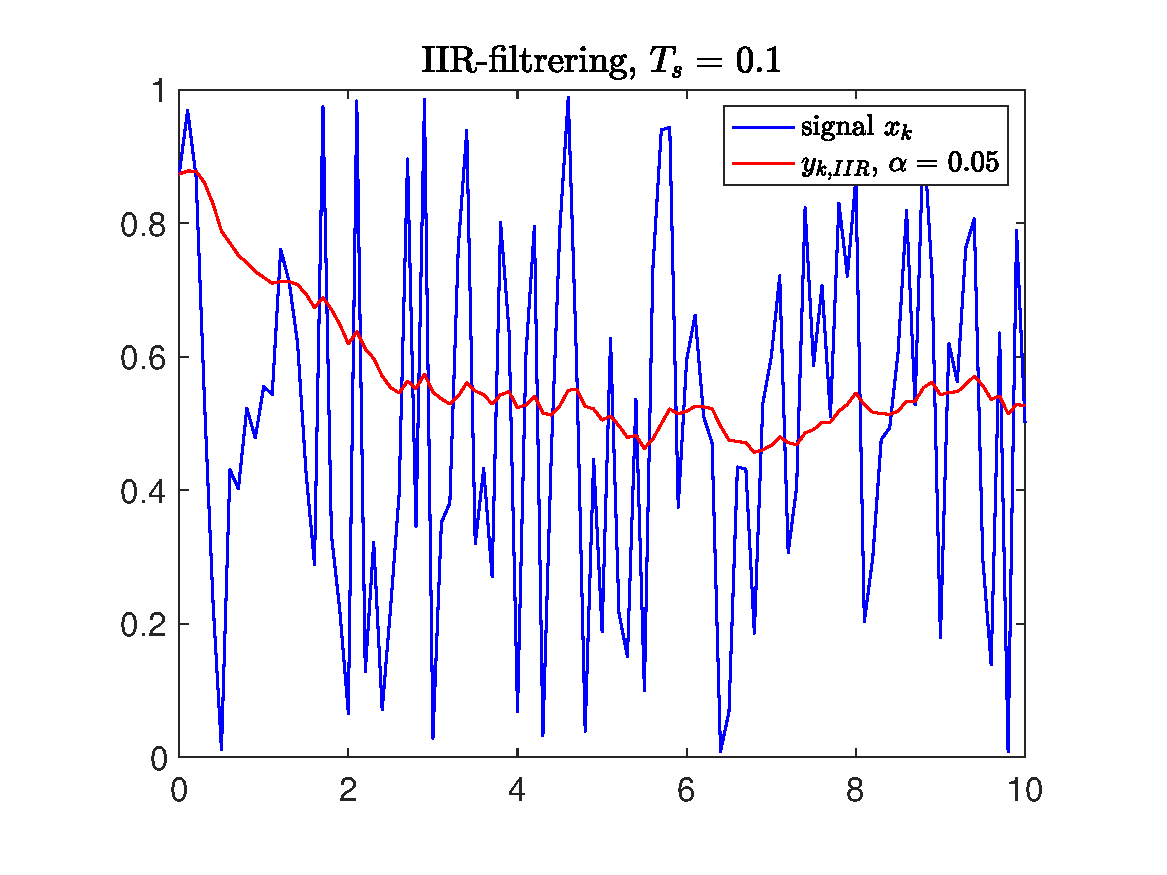
\includegraphics{3j.pdf}}
      \caption{Respons i IIR-filter med $\alpha{=}0.05$. }
      \label{fig:3j}
    \end{figure}
    
    
\item Innholdet i skallfilen \fbox{\tt IIR\_filter.m}  er vist under, 
og igjen brukes det beskrivende matematiske begrep for variabelnavn.

\begin{lstlisting}[caption={Skall for funksjonen for IIR-filtrering.},
 language= Matlab,   label=kode:IIR_funk, numbers=none, linewidth = 14.5cm] 
function FilteredValue = IIR_filter(OldFilteredValue, Measurement, para)
   % fyll inn
end
\end{lstlisting}
Ferdigstill koden i denne funksjonen.

\item Vis at du får samme   resultat som i figur~\ref{fig:3j} ved å
  endre {\it for}-løkken i skallfilen til 

\begin{lstlisting}[caption={Skall for funksjonen for IIR-filtrering.},
 language= Matlab,   label=kode:IIR_funk2,
 numbers=none]
 for k = 2:length(t)
    y_IIR(k) = IIR_filter(.., .., ..)
end
\end{lstlisting}

\subsubsection*{Effekten av $\alpha$}

\item For å teste betydningen av $\alpha$ så 
  er det i skallfilen {\tt oving3\_skallfil.m} laget til en egen
  seksjon som du kan kjøre direkte når du har laget ferdig funksjonen
  {\tt IIR\_filter}.    
Vis at du får resultatet vist i figur~\ref{fig:3j2}.

    \begin{figure}[H]
      \centering
      \hspace*{0mm}\scalebox{0.5}{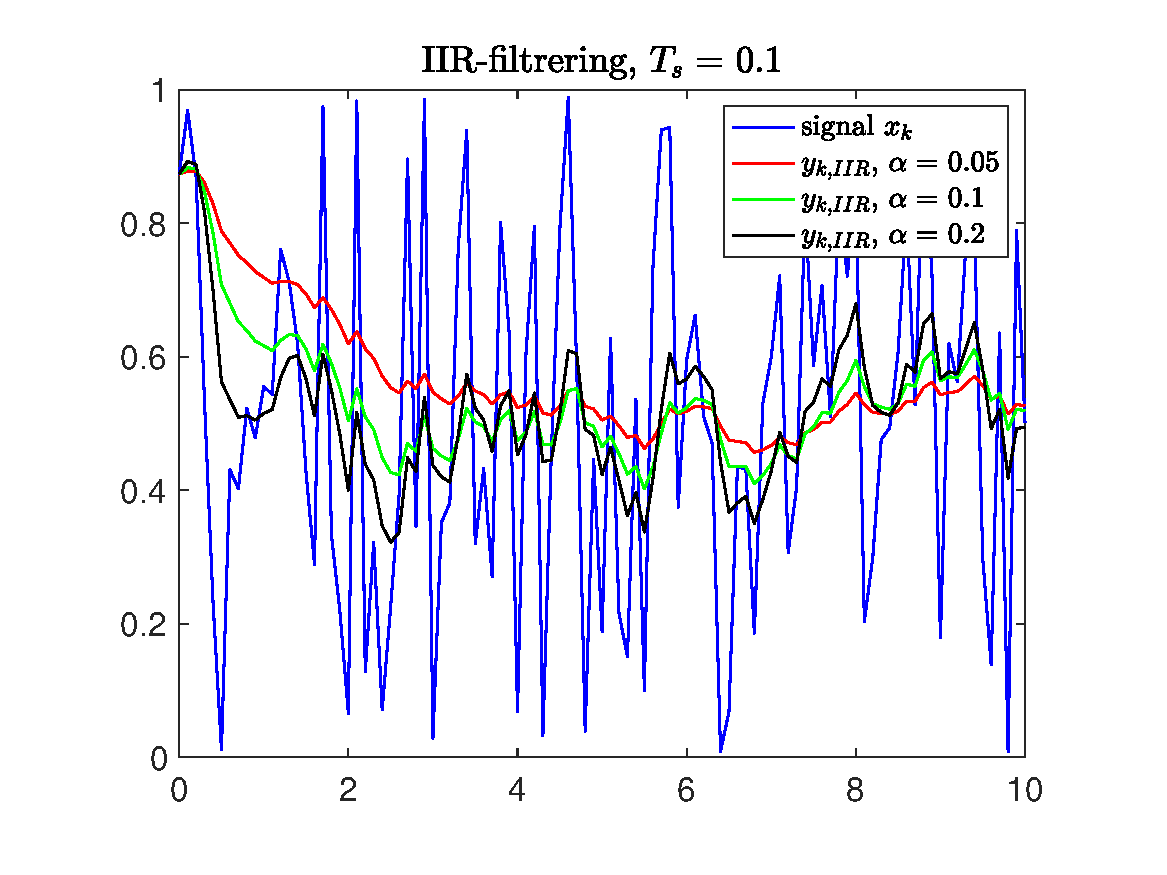
\includegraphics{3j2.pdf}}
      \caption{Respons i IIR-filter med $\alpha{=}[0.05, 0.1, 0.2]$. }
      \label{fig:3j2}
    \end{figure}

    \item   Er filtreringen som oppnås fornuftig i forhold til synkende tall på $\alpha$?

    \item Test ut $\alpha=0$ eller $\alpha=1$. Er
      resultatet fornuftig?

    \item Hva skjer dersom du setter $\alpha=-0.1$,  $\alpha=1.7$,
      $\alpha=2$ eller $\alpha=2.3$? Kan du forklare hva som skjer?

      
\end{itemize}
